\documentclass{standalone}
\usepackage{../preamble}

\begin{document}
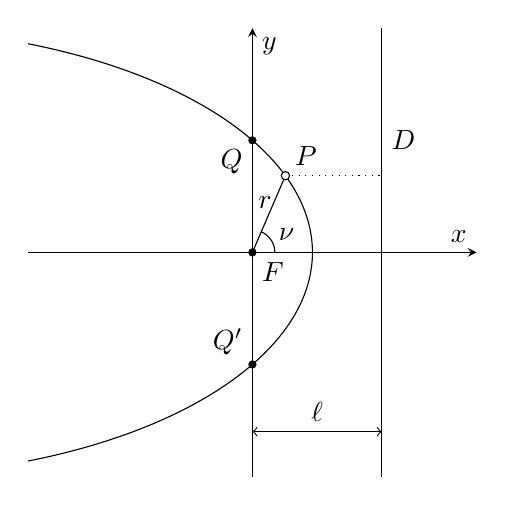
\begin{tikzpicture}
  \begin{axis}[
      xmin=-1,xmax=1,ymin=-1,ymax=1,
      axis lines=middle,
      ytick = {0},
      xtick = {0},
      axis equal image,
      ylabel={$y$},
      xlabel={$x$},
    ]
    \def\a{2}
    \def\b{1}
    \def\c{sqrt(\a^2-\b^2)}
    \def\ymax{\pgfkeysvalueof{/pgfplots/ymax}}
    \def\ymin{\pgfkeysvalueof{/pgfplots/ymin}}
    \addplot[thin,samples=400,domain=-80:80] ({\a*cos(x)-\c},{\b*sin(x)});
    \addplot[thin,samples=200,domain=\ymin:\ymax] ({\a^2/\c-\c},{x});

    \fill[black] (0,0) circle(1.5pt) node[anchor=north west]{$F$};
    \fill[black] (0,{\b^2/\a}) circle(1.5pt) node[anchor=north east]{$Q$};
    \fill[black] (0,{-\b^2/\a}) circle(1.5pt) node[anchor=south east]{$Q'$};
    \draw[thin,<->] (0,{-\b^2/\a-0.3}) -- ({\a^2/\c-\c},{-\b^2/\a-0.3}) node[anchor=south,pos=0.5]{$\ell$};
    \draw[thin,-] (0,0) -- ({\a*cos(20)-\c},{\b*sin(20)});
    \draw[thin,dotted] ({\a*cos(20)-\c},{\b*sin(20)}) -- ({\a^2/\c-\c},{\b*sin(20)});
    \draw[black, fill=white] ({\a*cos(20)-\c},{\b*sin(20)}) circle(1.5pt) node[anchor=south west]{$P$};
    \node[anchor=west] at ({\a^2/\c-\c},0.5){$D$};

    % angles
    \draw[domain=0:67,samples=100] plot ({0.1*cos(\x)}, {0.1*sin(\x)});
    \node[anchor=south west] at (0.075,0.01) {$\nu$};
    \node[anchor=south east] at (0.13,0.15) {$r$};
  \end{axis}
\end{tikzpicture}
\end{document}